\documentclass[conference, 11pt]{IEEEtran} 
\usepackage{verbatim}
\usepackage{multirow} \usepackage{enumerate}
\usepackage{amsmath,enumerate} \usepackage{amsthm}
\usepackage{algcompatible}
\usepackage{algpseudocode}
\usepackage{algorithm}
%\usepackage{algorithmic}
\usepackage{pstricks}
\usepackage{amssymb, latexsym}
\usepackage{xfrac}
\usepackage{mathtools}
\usepackage{graphicx}
\usepackage{subfig}
\DeclareGraphicsRule{*}{mps}{*}{}
\usepackage{listings}

%specific to this document only
\usepackage{pgfplots}
\usepackage{pgfplotstable}
\pgfplotstableread{plts/experiment8b1_av.tab}\averageone
\pgfplotstableread{plts/experiment8b2_av.tab}\averagetwo
\pgfplotstableread{plts/experiment8b3_av.tab}\averagethree
\pgfplotstableread{plts/experiment8b4_av.tab}\averagefour
\pgfplotstableread{plts/experiment9a_av.tab}\stepping
\pgfplotstableread{plts/experiment9a1_av.tab}\steppingone
\pgfplotstableread{plts/experiment9a2_av.tab}\steppingtwo
\pgfplotstableread{plts/experiment9a3_av.tab}\steppingthree
\pgfplotstableread{plts/experiment9a4_av.tab}\steppingfour
\pgfplotstableread{plts/experiment9b1_av.tab}\runningone
\pgfplotstableread{plts/experiment9b2_av.tab}\runningtwo
\pgfplotstableread{plts/experiment9b3_av.tab}\runningthree
\pgfplotstableread{plts/experiment9b4_av.tab}\runningfour
\pgfplotstableread{plts/experiment9b_av.tab}\running
\pgfplotstableread{plts/experiment9c_av.tab}\costcomp
\pgfplotstableread{plts/experiment9c1_av.tab}\costcompone
\pgfplotstableread{plts/experiment9c2_av.tab}\costcomptwo
\pgfplotstableread{plts/experiment9c3_av.tab}\costcompthree
\pgfplotstableread{plts/experiment8b1_rn.tab}\runsone
\pgfplotstableread{plts/experiment8b2_rn.tab}\runstwo
\pgfplotstableread{plts/experiment8b3_rn.tab}\runsthree
\pgfplotstableread{plts/experiment8b4_rn.tab}\runsfour
\pgfplotstableset{
  create on use/density/.style={
    create col/expr={\thisrow{nodes}+\thisrow{links}}}
    }
\pgfplotstableset{
  create on use/delta/.style={
    create col/expr={\thisrow{links}*2}}
    }
\pgfplotstableset{
  create on use/nodebylinks/.style={
    create col/expr={(\thisrow{nodes}*\thisrow{links})}}
    }
\pgfplotscreateplotcyclelist{three}{% 
  every mark/.append style={fill=teal}\\% 
  every mark/.append style={fill=green}\\% 
  every mark/.append style={fill=orange}\\% 
}
\pgfplotscreateplotcyclelist{four}{%
  every mark/.append style={fill=teal}\\%
  every mark/.append style={fill=green}\\%
  every mark/.append style={fill=orange}\\%
  every mark/.append style={fill=pink}\\%
}

%%%%%%%%%%%%%

\usepackage{pgf}
\usepackage{tikz}
\usetikzlibrary{decorations.pathmorphing} % LATEX and plain TEX when using Tik Z
\usetikzlibrary{positioning}
\usetikzlibrary{er}
\usetikzlibrary{automata}
\usetikzlibrary{shapes.geometric}
\tikzstyle{vx}=[draw,circle,fill=white,minimum size=2pt, inner sep=1pt, node distance=15mm]
\tikzstyle{ex}=[draw,rectangle,fill=white,minimum size=2pt, inner sep=3pt, node distance=15mm]
\tikzstyle{bup}=[semithick, decoration={bent, aspect=.3, amplitude=4}, decorate, ->, >=stealth]
\tikzstyle{bdn}=[semithick, decoration={bent, aspect=.3, amplitude=-4}, decorate, ->, >=stealth]
\tikzstyle{BUP}=[thick, decoration={bent, aspect=.3, amplitude=8}, decorate, ->, >=stealth]
\tikzstyle{BDN}=[thick, decoration={bent, aspect=.3, amplitude=-8}, decorate, ->, >=stealth]
\tikzstyle{MUP}=[thick, decoration={bent, aspect=.3, amplitude=16}, decorate, ->, >=stealth]
\tikzstyle{MDN}=[thick, decoration={bent, aspect=.3, amplitude=-16}, decorate, ->, >=stealth]
\tikzstyle{str}=[semithick, decorate, ->, >=stealth]
\tikzstyle{cr}=[draw, circle, fill=black!25,minimum size=150pt]

%styles for plots?
\tikzstyle{bls}=[blue, solid, mark=square*]
\tikzstyle{grt}=[red, solid, mark=*]
% \paperheight=11in \paperwidth=8.5in \textheight=9.0in
% \textwidth=6.5in \voffset=-.875in \hoffset=-.875in
\newenvironment{code} {\begin {quote}\begin{footnotesize}}
    {\end{footnotesize}\end{quote}}

% \oddsidemargin 0.0 in \evensidemargin 0.0 in
\newenvironment{enumeratealpha}
{\begin{enumerate}[(a{\textup{)}}]}{\end{enumerate}}

\theoremstyle{plain}
\newtheorem{lem-rule}{Rule}
\newtheorem{thm}{Theorem}
\newtheorem{lem}{Lemma}[thm]
\newtheorem{prop}{Proposition}[thm]
\newtheorem{lprp}{Proposition}[lem]
\theoremstyle{definition}
\newtheorem{defn}{Definition}[thm]
\newtheorem{dfn}{Definitions}[thm]
\newtheorem{ldef}{Definition}
\theoremstyle{remark}
\newtheorem{smy}{Summary}
\newtheorem{note}{Note}[thm]

%algorithms commands
\algblockdefx[Case]{Case}{EndCase} %
[1] [{\em var}] {{\bfseries case} {\em #1\ } } %
{{\bfseries end case}}%
\algcblockdefx[Case]{Case}{When}{EndCase}
[1] [{\em true}] {{\bfseries when} {\em #1\ }}
{{\bfseries end case}} %

\algblockdefx[TimesDo] {DoTimes}{EndTimes}
[1] [0] {#1 times {\bfseries do}}
{{\bfseries end do}}

%subalgorithms environment
\makeatletter
\newcounter{parentalgorithm}
\newenvironment{subalgorithms}{%
%  \refstepcounter{algorithm}%
  \floatname{algorithm}{Procedure}
  \protected@edef\theparentalgorithm{\thealgorithm}%
  \setcounter{parentalgorithm}{\value{algorithm}}%
  \setcounter{algorithm}{0}%
  \def\thealgorithm{\theparentalgorithm-\alph{algorithm}}%
  \ignorespaces
}{%
  \setcounter{algorithm}{\value{parentalgorithm}}%
  \ignorespacesafterend
}
\makeatother

%code environments
\usepackage{float}
 
\floatstyle{ruled}
\newfloat{codeblock}{thp}{lop}
\floatname{codeblock}{Example}

\lstnewenvironment{rubyblock} 
{\lstset{language=Ruby, basicstyle=\small, xleftmargin=10pt, numbers=left, numberstyle=\tiny, stepnumber=2, numbersep=5pt}}
{}
% text macros
\def\cI{{\mathcal I}} \def\cR{{\mathcal R}} \def\cE{{\mathcal E}}
\def\cC{{\mathcal C}} \def\cF{{\mathcal F}} \def\cU{{\mathcal U}}
\def\cH{{\mathcal H}} \def\cD{{\mathcal D}} \def\cB{{\mathcal B}}
\def\cQ{{\mathcal Q}} \def\cV{{\mathcal V}} \def\cS{{\mathcal S}}
\def\cG{{\mathcal G}} \def\cA{{\mathcal A}} \def\cO{{\mathcal O}}
\def\cW{{\mathcal W}} \def\cL{{\mathcal L}} 

\def\bI{{\mathbb I}} \def\bO{{\mathbb O}}
\def\bC{{\mathbb C}} \def\bM{{\mathbb M}}
\def\bId{{$\mathbb I$}} \def\bOd{{$\mathbb O$}}
\def\bCd{{$\mathbb C$}} \def\bMd{{$\mathbb M$}}

\def\cId{{$\mathcal I$}} \def\cRd{{$\mathcal R$}} \def\cEd{{$\mathcal E$}} 
\def\cCd{{$\mathcal C$}} \def\cFd{{$\mathcal F$}} \def\cUd{{$\mathcal U$}} 
\def\cHd{{$\mathcal H$}} \def\cDd{{$\mathcal D$}} \def\cBd{{$\mathcal B$}} 
\def\cQd{{$\mathcal Q$}} \def\cVd{{$\mathcal V$}} \def\cSd{{$\mathcal S$}} 
\def\cGd{{$\mathcal G$}} \def\cAd{{$\mathcal A$}} \def\cOd{{$\mathcal O$}}
\def\cWd{{$\mathcal W$}} \def\cLd{{$\mathcal L$}}

\bibliographystyle {IEEEtranS}

\begin{document}
\title{Distributed Vertex Cover in Network Graphs} 

\author{\IEEEauthorblockN{J. Paul Daigle and Sushil K. Prasad}
\IEEEauthorblockA{Department of Computer Science\\
Georgia State University\\
Atlanta, Georgia 30303, USA\\}
}

\maketitle

\begin{abstract}
 Vertex cover, a minimal set of nodes to cover all edges in a graph, is an abstraction of coverage problems in sensor networks, transportation networks, etc, and is a well-konwn NP-hard problem.  Minimum weighted vertex cover (MWVC) problem asks for further minimizing the cumulative weight of a vertex cover.  We present new distributed k-hop algorithms for MWVC problem with theoretical and practical values.  Our first 1-hop approximation algorithm, based on matching a maximal set of non-adjacent edges, is provably 2-optimal with a communication complexity of $O(\Delta)$.   It compares very well with the current state-of-art in quality while significantly reducing communication cost.

We also explore an important variant, the problem of finding a series of vertex covers to maximize network lifetime.  Our second algorithm, based on a key insight into the vertex cover problem of collecting partial covers from 2-hop neighbors, is an excellent practical algorithm.  It is representative of a problem-structure based efficient sampling algorithm in the exponential size local solution space.   We show that a partial cover based algorithm can be enhanced further to compete very well and exceed the lifetime obtained with state-of-the-art algorithms. 
\end{abstract}
\section{Introduction}
The Minimum Vertex Cover problem and its weighted variant are NP-Complete problems with several known linear time sequential algorithms that provide constant approximations. The existence of such algorithms suggests that there is a constant time distributed algorithm that would provide a constant approximation for MVC or MWVC, but it has been shown that a constant approximation of MWVC cannot be found by a distributed algorithm in a constant number of rounds\cite{1011811}. 

Here we present a distributed 2-optimal algorithm to solve MWVC in an expected running time of $O(\Delta)$, based on the linear time sequential algorithm of Gonzalez\cite{Gonzalez1995129}. In addition, we present an interesting subroutine that runs in constant time and improves the quality of solutions for both our algorithm and the prior algorithm of Koufogiannakis and Young\cite{1582746}. This subroutine turns out to have practical value when applied to the related problem of sensor network lifetime.

Definitions and descriptions of prior work is presented in Section~\ref{sec:background}. In Section~\ref{sec:algorithms} we describe our own distributed algorithms for both network lifetime and MWVC. Section~\ref{sec:simulator} contains the description of our simulation software design, which provides the engine for the experiments that are described in Section~\ref{sec:experiments}.

\section{Background}
\label{sec:background}
\subsection{Definitions}
The coverage problems in this paper are common coverage problems which are known to be NP-Complete. For convenience, the problem definitions are provided here.

\subsubsection{Minimum Vertex Cover (MVC)}
\label{sub:mvc}
Given an undirected Graph $G(V,E)$, a {\em Vertex Cover} of $G$ is a set of vertices $V'$ such that for each edge $e_{u,v} \in E$, $u \in V'$ or $v \in V'$. The Minimum Vertex Cover Problem is to find the smallest possible vertex cover of $G$.

\subsubsection{Minimum Weighted Vertex Cover (MWVC)}
\label{sub:mwvc}
Given an undirected Graph $G(V,E)$, where each $v \in V$ has a positive weight $w(v)$, minimize $\sum_{v \in V'} w(v)$.

%\subsubsection{Minimum (Weighted) Vertex Cover of a Hypergraph}

%Given a Hypergraph $G(V,E)$, with vertices $v \in V$ and hyperedges $e_{v_1...v_n}$, a vertex cover of $G$ is a set $V'\: | \: \forall e \in E,\quad \exists v \in V'\: |\: v \in e$. The minimum vertex cover and minimum weighted vertex cover are as described in sections~\ref{sub:mvc} and ~\ref{sub:mwvc}

\subsubsection{Network Lifetime}
\label{sub:mvc}
Given a sensor network $N(S,T)$, the {\em Network Lifetime} of $N$ is the maximum time that $\forall t \in T, \exists s \in S | s{\text \ covers\  } t$.

\subsubsection{Model}
\label{ssb:com-model}

All of the distributed algorithms described are assumed to be running on a {\em message passing model}, the compute nodes are mapped to the vertices of the graph, and the edges of the graph represent viable paths for communication between nodes. 

\subsection{Prior Work}

Sequential Linear time algorithms for covering problems are surveyed in detail in \cite{254190}. The seminal paper on Linear Programming techniques for constant ratio approximation of MWVC was published by Bar-Yehuda and Even in 1981 \cite{Bar-Yehuda:1981lr}. Gonzalez created a 2-optimal LP-Free linear time algorithm based on Maximal Matching in 1995 which is the basis of our distributed algorithm \cite{Gonzalez1995129}. 

We are aware of two distributed algorithms for minimum weighted vertex cover. A 2-optimal algorithm based on maximal matching was published in 2008 by Grandoni et. al \cite{1435381}. We implement a simpler algorithm presented by Koufaganis and Young in 2009 for performance comparison \cite{1582746}. The Koufaganis/Young algorithm is described in detail in Section~\ref{sec:k-y-alg}.

The network lifetime problem is introduced in detail by Cardei et. al in \cite{1498475}. A mathematical analysis of the problem is provided by Legakis et all in \cite{4697802}. Brinza and Zelikovski's deterministic algorithm \cite{1640702}, detailed in Section~\ref{sec:deeps} is used in this paper as a point of comparison. The issue of communication costs is addressed by Zhao et. all, along with a formal definition for the {\em Connected Target Coverage Problem}\cite{1514028}. Dhawan and Prasad introduce the use of Dependency Graphs for the network lifetime problem in \cite{978-3-540-77220-0_36}, this work provides the jumping off point for the algorithm introduced in Section~\ref{sec:PCDG}. Dependency Graphs are explored further in Section~\ref{sec:dep-graphs}.

\subsection{The Koufaganis/Young Algorithm}
\label{sec:k-y-alg}

The Koufaganis/Young Algorithm (K/Y) described in this paper is the $O(\log n)$ 2-optimal distributed algorithm for the Minimum Weighted Vertex Cover published by Koufaganis and Young in 2009\cite{1582746}. The algorithm improves on the previous best known distributed algorithm for MWVC, which runs in $O(\log n + \log W)$, where  $W$ is the average vertex weight\cite{1435381}.

The K/Y algorithm uses a special variable, maintained by each vertex $v$, referred to as $x_v$ and initialized to 0. Each vertex decides whether or not to join the cover by calling a subroutine, {\ttfamily step}, which takes as inputs the current value of $x_v \text{ and } x_w$ and the weights $c_v \text{ and } c_w$. {\ttfamily step} updates the value of x by Equation~\ref{eqn:step}.

\begin{align}
  \label{eqn:step}
  \beta = min 
  \begin{dcases} 
    c_v(1 - x_v) \\
    c_w(1 - x_w)
  \end{dcases} \nonumber \\ 
  for (v, w), x_1 = x_0 + \frac{\beta}{c}
\end{align}

If $x \equiv 1 $ for $v \text{ or } w$, that vertex is added to the cover.

In each round, a node decides whether it will choose to be a {\em root} or a {\em leaf} node. If a node chooses to be a leaf node, it chooses among it's neighbors which are roots those which would {\em not} be added to the cover, if the {\ttfamily step} subroutine were run with the current value of x. From these, it chooses a random neighbor for this round, marking the appropriate edge as a {\em star edge}.

Root nodes collect their star edges and then choose to do one of the following: either run {\ttfamily step} for all star edges in some sequence, or run {\ttfamily step} for only the last star edge in the sequence. 

Each communication round is therefore made up of 3 communication steps. Each vertex must communicate to its neighbors whether it is a leaf or a root, then each leaf must communicate to the appropriate neighbor that they share a star edge, then each root must communicate the results of its choices to it's neighbors.


\subsection{The DEEPS Algorithm}
\label{sec:deeps}

The Deterministic Energy-Efficient Protocol for Sensor networks (DEEPS) provides a distributed algorithm for extending the lifetime of wireless sensor networks\cite{1640702}. DEEPS works by maintaining information about the total battery life of all sensors covering a given target. Targets are divided into {\em sinks} and {\em hills}. 

Sinks are defined as follows: if $b_t$ is the cumulative battery life of all sensors covering some target $t$, if for some sensor $s$ which covers $t$, $b_t$ is minimum for all targets covered by $s$, $t$ is a sink. Any target which is not a sink is a hill.

In order to avoid having a target abandoned, one sensor that covers a given target is placed in charge of that target. Sensors that are in charge of targets will not turn off unless another sensor covering that target turns on. 

The DEEPS protocol is a two-hop protocol, as each sensor needs to know not only the battery supplies of its own targets, but also the battery supply of all of its neighbors targets. It performs well against other scheduling protocols. 

\subsection{Dependency Graphs}
\label{sec:dep-graphs}

 The solution space for both of the problems addressed in this work is exponential to the input. A {\em Dependency Graph} is a strategy based on the insight that, from a strictly local standpoint, the input size of a graph problem remains constant regardless of the problem size. For a distributed system such as a sensor network, the space of all local solutions is only dependent on the size of the local neighborhood, not the size of the graph overall\cite{978-3-540-77220-0_36}. Prasad and Dhawan develop a framework for using Dependency Graphs in \cite{IPDPS.2008.45361}.

The framework applies to problems where local solutions can be combined to form a feasible global solution. The essential steps of the framework are as follows. 
\begin{enumerate}
\item Establish that combined local solutions lead to a feasible global solution.
\item Model the state space of the local solutions. \label{en:frame-model}
\item Determine a priority heuristic for local solutions.\label{en:frame-priority}
\item Design a reasonable negotiating strategy between neighbors.
\end{enumerate} 

The definition of the dependency graph is captured by step~\ref{en:frame-model}. Each local solution is considered a node in the Graph, and edges are defined by dependencies between solutions. Solutions and relationships between solutions might be directed, undirected, weighted, unweighted, and so forth. In step~\ref{en:frame-priority}, these parameters are used to determine what solutions are preferred. 

This framework has been applied to sensor network lifetime, and competes very well against other methods\cite{Dhawan:hipc-09}.

\section{Algorithms}
\label{sec:algorithms}
\label{sub:algorithms-dgmm}
\subsubsection{Description}
Algorithm~\ref{alg:dgmm} is our distributed implementation of the 2-optimal minimum weighted vertex cover algorithm presented by Gonzalez.\cite{Gonzalez1995129} The Gonzalez algorithm proceeds by selecting each edge in turn and choosing one of the endpoints of that edge to add to the cover. The sequential algorithm goes through each edge in turn and assigns the edge a weight according to equation~\ref{eqn:gmm}. If the weight of a vertex is equal to the sum of it's incident edge weights, that vertex is added to the cover. 

\begin{equation}
  \label{eqn:gmm}
  w(e(u,v)) = min 
  \begin{dcases} 
    w(u) - \sum_{i \ne v} w(e(u,i)) \\
    w(v) - \sum_{i \ne u} w(e(i,v)) 
  \end{dcases}    
\end{equation}

The distributed version of the algorithm chooses some disjoint set of edges and assigns weights as described. The precise method of choosing edges and updating weights is given in Algorithm~\ref{alg:dgmm}. The automaton capturing the state transitions of Algorithm~\ref{alg:dgmm} is given succinctly in Figure~\ref{fig:dgmm-auto}. Each vertex begins in the \cCd\ state, and chooses to either send invitations (\cId), or listen for invitation (\cLd). Vertices in the \cId\ state choose one neighbor to send an invitation to and transition to a waiting state (\cWd), and vertices in the \cLd\ state choose one invitation to accept. The acceptence message is sent during the response state \cRd. All vertices then update their status (\cUd). Vertices that have either chosen to join the cover or which have no undecided neighbors will transition to the done state, (\cDd), and other vertices return to state \cCd.  

\begin{figure}[htp]
  \caption{DGMM Automata}
  \begin{center}
  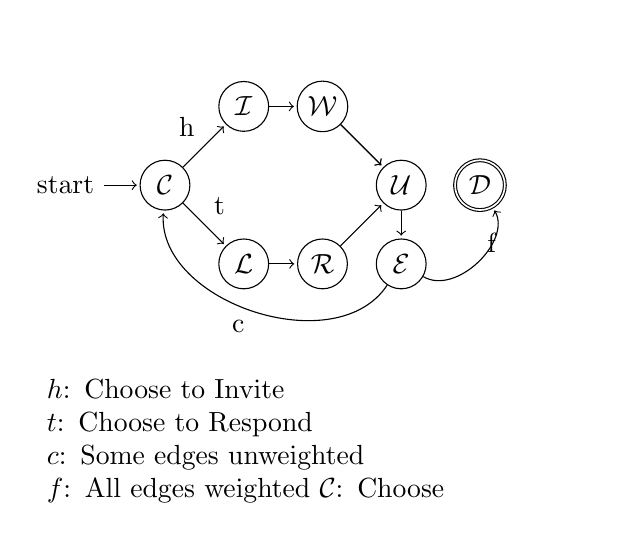
\begin{tikzpicture}[shorten >=1pt,node distance=1cm,on grid,auto, bend angle=75, every state/.style={scale=1, minimum size=18pt, inner sep=2pt}]
    %\draw [help lines] (0,-2) grid (4,2);
    \path [help lines] (0,-2) grid (4,2); 
    \node [state, initial]   (C)          {\cCd};
    \node [state] (I)            at (1,1) {\cId};
    \node [state] (L)            at (1,-1) {\cLd};
    \node [state] (W)            at (2,1)       {\cWd};
    \node [state] (R)            at (2,-1)       {\cRd};
    \node [state] (U)            at (3,0) {\cUd};
    \node [state] (E)            at (3,-1)       {\cEd};
    \node [state, accepting] (D) at (4,0)   {\cDd};

    \path [->] (C) edge              node {h} (I)
                   edge              node {t} (L)
               (L) edge              node {} (R)
               (I) edge              node {} (W)
               (W) edge              node {} (U)
               (R) edge              node {} (U)
               (U) edge              node {} (E);
    \path [->] (E) edge [bend right] node [above right] {f} (D);
    \path [->] (W) edge              node {} (U);
    \path [->] (E) edge [bend left]  node {c} (C);


      \node [text width=7cm] (key) at (2, -3.25) {
	$h$: Choose to Invite \hspace{4cm}
        $t$: Choose to Respond\hspace{4cm}
        $c$: Some edges unweighted\hspace{5cm}
	$f$: All edges weighted
	$\cC$: Choose 
	}; 
  \end{tikzpicture}
  \end{center}
  \label{fig:dgmm-auto}
\end{figure}


During the \cUd\ state, vertex pairs formed during the invitation/acceptance phases are able to assign a weight to the edge between them independently using equation~\ref{eqn:gmm}, and therefore decide whether or not to join the cover. During the \cEd\ state neighboring vertices are able to update some of their own edge weights, by assigning a weight of zero to any edges incident to a vertex which has joined the cover.

\begin{algorithm}
\caption{Distributed Weighted Vertex Cover}
\begin{algorithmic}
\Require {$G(V,E)$: a graph}
\ForAll {$v_u \in V$ in parrallel}
\State $S_u \leftarrow False$
\State state $\leftarrow$ Choose
\Repeat
\State Broadcast $S_u$
\If {$S_v = True$ for $v_v$ incident to self}
\State Set Weight $e_{u,v} \leftarrow 0$
\EndIf
\If {state = Choose}
\State {Choose A State (Invite, Listen)}
\ElsIf {state = Invite}
\State {Select an unweighted edge, $e_{u,v}$}
\State {Broadcast an Invitation to $v_v$}
\State {state $\leftarrow$ Wait}
\ElsIf {state = Listen}
\State {Collect Invitations}
\State {state $\leftarrow$ Respond}
\ElsIf {state = Wait}
\State {Collect Responses}
\If {Response Matches Invitation}
\State {Update Weight $e_{u,v}$}
\If {$\sum_{w_e} e incident v_u = w_u$}
\State $S_u \leftarrow true$
\EndIf
\EndIf
\State {state $\leftarrow$ Choose}
\ElsIf {state = Respond}
\State Choose Invitation, Broadcast Response
\State {Update Weight $e_{u,v}$}
\If {$\sum_{w_e} e incident v_u = w_u$}
\State $S_u \leftarrow true$
\EndIf
\State {state $\leftarrow$ Choose}
\EndIf
\Until {$S_u = true$ OR $S_v = true$ for all $v_v$ incident $v_u$}
\EndFor
\end{algorithmic}
\label{alg:dgmm}
\end{algorithm}

\subsubsection{Performance}

Our experiments show that DGMM finds covers that are equivalent to those found by other 2-optimal algorithms, in far fewer communication rounds. A formal proof supporting our experimental results follows.

\begin{thm}
  Algorithm~\ref{alg:dgmm} (DGMM) will always generate a 2-optimal cover in $O(\Delta)$ communication rounds.
\label{thm:dgmm-term}
\end{thm}
\begin{smy}
We show first that our algorithm conducts the same steps in the same order as a sequential algorithm that is known to produce a 2-optimal result, next that the algorithm will terminate in $O(\Delta)$ communication rounds.
\end{smy} 

\begin{note}[Communication Model]
\label{not:com-model}
As mentioned in Section~\ref{ssb:com-model}, we assume a message passing model of distributed computing. In each communication round, it is assumed that every node can communicate with its neighbors. Communication is assumed to be synchronous and symetric: if node $a$ is a neighbor of node $b$, node $b$ is a neighbor of node $a$, and if node $a$ has counted $x$ communication steps, so has node $b$.

A ``communication round'' is actually three steps: an invitation sending step, an information response step, and an exchange step where neighbors share changes in status.\footnote{It should be noted that the K/Y algorithm also requires three communication events per round.} 
\end{note}
\begin{note}[Local Information]
\label{not:dgmm-local-info}
At the beginning of each communication round, each node has a list of it's neighbors, their current state, the edges associated with those neighbors, and the results of any previous computation performed on those edges.
\end{note}
\begin{note}[Mapping to Sequential Algorithm]
\label{not:gmm-dgmm}
DGMM is based on a sequential algorithm (GMM), which takes as an input a graph and produces a 2-optimal vertex cover of that graph. The sequential algorithm selects each edge of the graph in turn, in arbitrary order, and compares the endpoints of that edge. The edge is assigned a weight according to Equation~\ref{eqn:gmm}. If one endpoint is already in the cover, the resulting weight will be zero, otherwise, one endpoint will be added to the cover. When each edge has been assigned a weight, the algorithm terminates and outputs the cover.

For DGMM, the Graph is represented as a network of compute nodes, with the nodes representing vertexes and connections between the nodes representing edges. Nodes form pairs over these connections and weight them, following the same rules as the sequential algorithm. Nodes turn off if they have no unweighted edges and have not joined the cover. When the algorithm terminates, every node in the network that is in the cover will be in an ``on'' state, and every node that is not will be in an ``off'' state.
\end{note}
\begin{proof}[Proof of Theorem~\ref{thm:dgmm-term}]
\label{prf:correct}

\begin{lem}
\label{lem:dgmm-edge}
  DGMM weights each edge once in a manner equivalent to GMM.
\end{lem}
\begin{proof}[Proof of Lemma~\ref{lem:dgmm-edge}]
  Lemma~\ref{lem:dgmm-edge} can be restated in terms of the following propositions.
  \begin{lprp}
    \label{prop:dgmm-edge-order}
    Given a matching, a simultaneous weighting of that matching is equivalent to any sequential weighting.
  \end{lprp}
  \begin{lprp}
    \label{prop:dgmm-edge-match}
    DGMM produces a matching in each communication round.
  \end{lprp}
  \begin{lprp}
    \label{prop:dgmm-edge-once}
    DGMM weights every edge exactly once.
  \end{lprp}
  If these propositions are true, Lemma~\ref{lem:dgmm-edge} is also true. 
  
  \begin{proof}[Proof of Proposition~\ref{prop:dgmm-edge-order}]
    Equation~\ref{eqn:gmm} for weighting an edge $e(u,v)$ is 
    \begin{equation*}
      weight(e(u,v)) = min
      \begin{dcases}
        \sum_{i \ne v} weight(e(u,i))\\
        \sum_{i \ne u} weight(e(v,i))
      \end{dcases}
    \end{equation*}
    By definition of a matching, no two edges in a matching share a vertex. Therefore, if an edge $e(u,v)$ is in the matching, no edge $e(u,i)$ is in the matching. 
    Take a matching \bMd\ in a Graph $G(V,E)$, composed of edges $\{e_0, e_1, ..., e_n\}$ If we use the sequential algorithm to weight the edges in \bMd\ one after the other, it is obvious that no edge outside of \bMd\ will change. Since only edges outside of \bMd\ are used to assign weights to edges inside \bMd\, it does not matter what order the weights are assigned in, or whether the weight assignment occurs to all edges in \bMd\ simultaneously.
    
    Therefore Proposition~\ref{prop:dgmm-edge-order} is true.
  \end{proof}
  \begin{proof}[Proof of Proposition~\ref{prop:dgmm-edge-match}]
    Assume not, that is, assume that there are two edges $e(u,v) \text{ and } e(i,v)$ that are both updated during the same communication round. For this to happen, some compute node $v$ must form a partnership with two nodes $i$ and $u$. 
    At the beginning of every communication round, each node makes an equally weighted random decision to either issue an invitation or wait for invitations. We consider these options by cases.
    Case One: Assume that $v$ issues invitations. If $v$ issues invitations, $v$ will choose a single unweighted edge $(v,u)$ and broadcast an invitation with the id of $u$ to all of it's neighbors (Line~\algref{alg:dgmm}{alglin:dgmm-issue-invite}). $v$ then transitions to the \cWd\ state. In this state, the node gathers all responses issued by its neighbors, and updates an edge if a response is sent specifically to itself.
    So if two edges are weighted, $v$ must receive two responses.
    Responses are issued by nodes in the \cRd\ state. Each node in this state chooses a single invitation from it's received invitations and responds to it. Since $v$ gets two responses, therefore, $v$ must have invited two separate nodes in this round. But $v$ only issued one invitation, so this is a contradiction.
    Case Two: Assume that $v$ receives invitations. Since $v$ is weighting two edges, $v$ must respond to multiple invitations in this round. However, according to the algorithm, $v$ only sends a single response message, which is a contradiction as well.
    Therefore, Proposition~\ref{prop:dgmm-edge-match} is true.
  \end{proof}
  \begin{proof}[Proof of Proposition~\ref{prop:dgmm-edge-once}]
    Because a node will only attempt to weight an unweighted edge, we know that no edge will be weighted more than once. If the proposition is false, it must be the case that some edge is not weighted.
    For an edge to be unweighted, both endpoints of the edge would have to halt (enter the \cDd\ state) before the edge is weighted. Nodes halt under two circumstances:
    \begin{enumerate}
    \item The node has joined the cover.
    \item A nodes neighbors have all joined the cover.
    \end{enumerate}
    In the first case, the node will weight all of it's unweighted edges to 0. In the second case, the node weights it's own edges to 0 if the other endpoint is in the cover.
    Therefore, if the algorithm halts, all edges have been weighted once.
  \end{proof}
  Therefore, Lemma~\ref{lem:dgmm-edge}.
\end{proof}

\begin{lem}
  \label{lem:dgmm-delta}
  DGMM will weight all edges in approximately $2\Delta$ communication rounds.
\end{lem}
\begin{proof}[Proof of Lemma~\ref{lem:dgmm-delta}]

Following the automata in Figure~\ref{fig:dgmm-auto}, each communication round starts with a choice phase (labeled \cCd), after which the nodes will be divided approximately in half, with half being senders in the next round and half being recievers. A given node $u$, then, will become a reciever (indicated by state \cLd) with a probability of $\frac{1}{2}$. The degree of $u$ can be assumed, without loss of generality, to be the maximum degree in the graph, indicated as $\Delta$. 

Roughly half of the neighbors of $u$ will be senders (indicated by state \cId). For each of these, we can assume a degree of $\Delta$ as well, meaning that for each neighbor $v$ of $u$, there is a probability of $\frac{1}{\Delta}$ that $v$ will invite $u$ to weight edge $(u,v)$ in this round. Since $u$ has $\frac{\Delta}{2}$ neighbors that are also senders, $u$ will recieve an invitation with a probability of $\frac{1}{2}$. 

Therefore, in any given round, roughly $\frac{1}{4}$ of the total number of nodes will recieve an invitation from a neighbor to weight an edge. Each node that recieves at least one invitation will reply to exactly one invitation. The inviting node and the invited node together form the endpoints of an edge, which will be weighted in that communication round. So approximately $\frac{1}{2}$ of the total number of nodes will weight one edge in each communication round.

A node that weighted an edge in each communication round would weight all of it's edges in $\Delta$ rounds. By the reasoning above, each node will weight an edge in a round with probability of $\frac{1}{2}$, so we can expect that every node in the graph will complete weighting all of its edges after approximately $2\Delta$ communication rounds.

\end{proof}
\begin{lem}
  \label{lem:dgmm-cover}
  If an edge is weighted, at least one endpoint must be in the cover.
\end{lem}
\begin{proof}[Proof of Lemma~\ref{lem:dgmm-cover}]

  Suppose that Lemma~\ref{lem:dgmm-cover} is not true, so an edge is weighted, but neither endpoint is in the cover. For this to happen, two nodes that are not in the cover would have to form an exclusive node pair and evaluate a previously unweighted edge between them in some communication round, because the formation of such a partnership is a necessary precursor to evaluating an edge in Algorithm~\ref{alg:dgmm} and such partnerships are exclusive by Lemma~\ref{lem:dgmm-delta} and form a matching by Lemma~\ref{lem:dgmm-edge}. 

  Edges are evaluated according to Equation~\ref{eqn:gmm}. To recall, this equation is a function which evaluates to the minimum, between nodes $u$ and $v$, of the weight of the node minus the sum of the weights of the weighted edges of the node. The result is then applied as the weight of the edge $(u,v)$. This weight is applied line~\algref{alg:dgmm}{alglin:dgmm-update-weight-R} or~\algref{alg:dgmm}{alglin:dgmm-update-weight-W}, so both nodes use the same inputs on the same equation to weight the same edge.

  Next, both nodes run a test in line~\algref{alg:dgmm}{alglin:dgmm-join-cover-R} or~\algref{alg:dgmm}{alglin:dgmm-join-cover-W} to determine whether to join the cover. If the sum of the weights of the edges of $u$ are equal to the weight of $u$, $u$ joins the cover.

  So if an edge becomes weighted but neither endpoint joins the cover, it must be the case that for both nodes $u$ and $v$, the sum of the edge-weights is not equal to the sum of the weight.

  We know that the weight of $e(u,v)$ is equal to the minumum, between $u$ and $v$, of the weight of the node minus the sum of the nodes edges. Without loss of generality, assume that the relevant node is $u$. We will use $w$ to refer to the weight of $u$, and $s$ to refer to the sum of the weights of all edges of $u$ except $e(u,v)$. Assume that the value of $w - s$ is $x$. Therefore, the weight applied to $e(u,v)$ is $x$. Since $u$ is not in the cover, however, we know that: 
\begin{equation*}
w-s = x \land w \ne x+s
\end{equation*}
Which is a contradiction.

Therefore, if an edge is weighted, at least one endpoint will be in the cover.
\end{proof}

Therefore, because DGMM weights all edges and assigns nodes to the cover in a manner equivalent to GMM in $O(\Delta)$ communication rounds, Theorem~\ref{thm:dgmm-term} is correct.
\end{proof}



\subsection{Redundancy Checking}
\label{sec:redundant}
When vertices make local decisions to join a cover, it is difficult to judge whether any neighbor will also decide to join the cover. In some cases, this leads to vertices joining the cover which can be subsequently removed while still retaining full coverage. Removing these nodes will certainly reduce the total weight of the cover. We therefore implement a {\em redundancy checking} algorithm. Figure~\ref{fig:red} shows the progression of Algorithm~\ref{alg:red}.

\begin{figure}[htp]
  \begin{center}
    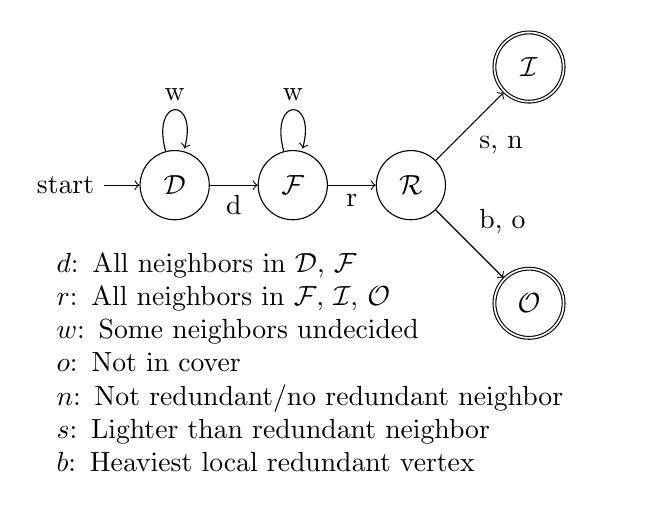
\begin{tikzpicture}
     % \draw[help lines] (0, -2) grid (5,2);
      \path [help lines] (0, -2) grid (5,2);
      \node [state, initial] (D) {\cDd};
      \node [state] (F) at (1.5, 0) {\cFd};
      \node [state] (R) at (3, 0) {\cRd};
      \node [state, accepting] (I) at (4.5, 1.5) {\cId};
      \node [state, accepting] (O) at (4.5, -1.5) {\cOd};

      \path [->] (D) edge node [below] {d} (F)
                     edge [loop above] node {w} ()
                 (F) edge node [below] {r} (R)
                     edge [loop above] node {w} ()
                 (R) edge node [above right]{b, o} (O)
                     edge node [below right]{s, n} (I);
      \node [text width=7cm] (key) at (2, -2.25) {$d$: All neighbors in \cDd, \cFd \hspace{4cm}
        $r$: All neighbors in \cFd, \cId, \cOd  \hspace{4cm}
        $w$: Some neighbors undecided  \hspace{5cm}
        $o$: Not in cover \hspace{5cm}
        $n$: Not redundant/no redundant neighbor  \hspace{4cm}
        $s$: Lighter than redundant neighbor  \hspace{4cm}
        $b$: Heaviest local redundant vertex  \hspace{4cm}};
                     
    \end{tikzpicture}
    \caption{Redundancy Checking Algorithm}
    \label{fig:red}
  \end{center}
\end{figure} 

\begin{algorithm}
\caption{ Redundancy checking algorithm (RC)} 
\begin{algorithmic}[1]
  \Require {$G(V,E), w(v)$: A vertex-weighted graph}
  \Require {state$(v_v) =  \cD \vee \cF$} \Comment See Fig~\ref{fig:red}
  \Ensure {state$(v_v) = (\cI \vee \cO)$}
  \ForAll {$v_v \in V$ synchronously}
  \If {state $=$ \cDd}
  \State {DO check-finished}
  \ElsIf {state $=$ \cFd}
  \State {DO check-redundant}
  \EndIf
  \EndFor
  \Procedure{check-finished}{}
  \If {$\forall v_u$ incident $v_v$, state$(v_u) = \cD \vee \cF$}
  \If {$v_v \in \bC$} \Comment Where \bCd\ is the Cover
  \If {$\forall v_u$ incident $v_v, v_n \in \bC$}
  \State {redundant $\gets$ TRUE}
  \EndIf
  \State {state $\gets$ \cFd}
  \EndIf
  \Else 
  \State {state $\gets$ \cDd}
  \EndIf
  \EndProcedure
  \Procedure{check-redundant}{}
  \If {$\forall v_u$ incident $v_v$, state$(v_u) = \cF \vee \cI \vee \cO)$}
  \If {redundant $=$ TRUE}
  \If {$\forall v_u$ incident $v_v$, redundant$(v_u) =$ FALSE}
  \State {remove $v_v$ from \bCd}
  \Else
  \State {$a \gets [w(v_v)] + [w(v_u) \forall v_u$ incident $v_v]$}
  \If {maximum of $a = v_v$} \Comment {$v_v$ has the largest weight in its neighborhood}
  \State {remove $v_v$ from \bCd}
  \EndIf
  \EndIf
  \EndIf
  \State {state $\gets \cI \vee \cO$}
  \Else
  \State {state $\gets$ \cFd}
  \EndIf
  \EndProcedure
\end{algorithmic}
\label{alg:red}
\end{algorithm}


The redundancy checking algorithm proceeds stepwise, similar to Algorithm~\ref{alg:dgmm}, and many of the same arguments apply. One difference is that redundancy checking is run a single time for each node, nodes check with their neighbors once and then decide to turn off only if they are the largest redundant node in their immediate neighborhood. Because no two neighboring nodes can both be the largest--assuming a tie breaking mechanism such as unique ids--such a decision cannot break the cover. Also, because nodes make the decision simultaneously and globally, the additional number or communication rounds required is constant.

The concept behind Algorithm~\ref{alg:red} is simple: A vertex is redundant if all of its neighbors are in the cover. This simple idea provides some valuable results extending network lifetime without incurring large communication costs, as we see later in Section~\ref{sec:pcdg-alg}. When examining target coverage in a sensor network, most current algorithms ignore the communication cost of establishing the target cover\cite{1514028}. One reason for this is that the cost is generally considered to be a constant, that is, any algorithm that provides continuous coverage must perform a global reshuffle periodically in order to maximize network lifetime. 

\subsection{Partial Cover Dependency Graph}
\label{sec:life-depend}
Network Lifetime and Minimum Weighted Vertex Cover are both NP-Complete problems. It has also been proved that MWVC cannot be approximated to a constant factor locally within any constant number of communication rounds~\cite{1011811}. This limitation must apply to target coverage as well. We developed our algorithm continuously covering the edges for extending total network lifetime based on the Dependency Graph which provides an algorithmic framework for target coverage and related problems~\cite{IPDPS.2008.45361}. 

The application of the framework relies on dependencies between local solutions. In the case of the vertex cover problem, there are several approaches that can be taken to determine what a local solution is. The simplest approach is to have each vertex only consider edges incident to itself. Naively, each vertex would have exactly two local solutions, the cover containing itself and the cover containing all of its neighbors. These two covers are node disjoint and lack any dependencies to prioritize meaningfully.   Therefore, one may consider the vertex covers for edges incident to 1-hop neighbors as well. Now a large number of possible covers have to be considered. The number of possible local covers for a vertex of degree $\Delta$ is $\sum_{i=0}^\Delta \binom{\Delta}{i}$. 

\label{sec:PCDG}
The number of local covers increases as a function of the density of the local neighborhood. If $\Delta$ is small, this is not a problem, but as $\Delta$ increases the number of potential local covers increases rapidly. The Partial Cover Algorithm samples this exponential space and reduces the number of solutions to O($\Delta$). A given vertex can only see two covers for it's own edges: the cover containing itself, and the cover containing all of its neighbors. The partial cover algorithm samples the solution space based on what vertices would have to be on if either of these two covers were off. 

\subsubsection{Construction of the  Partial Cover Dependency Graph (PCDG)}

Given a graph $G(V,E)$, for each vertex in $V$ we can define a partial cover dependency graph consisting of the {\em partial cover pair} $\bC_v, \bC_{n(v)}$ for v, and the partial cover pair for each neighbor of v. Given a node $v \in V$, $\bC_v$ consists of v and its two-hop neighbors, while $\bC_{n(v)}$ consists of $v$'s one-hop neighbors. Two nodes are connected (dependent), if the covers are non-disjoint. For clarity, we define terms below.

\begin{defn}
$N_v$ : The set of one-hop neighbors of $v$
\end{defn}
\begin{defn}
$N_v^2$ : The set of two-hop neighbors of $v$ 
\end{defn}

\begin{defn}
$\bC_v$ : $\{v\} \cup N_v^2$
\end{defn}

\begin{defn}
$\bC_{n(v)}$ : $N_v$
\end{defn} 

\begin{defn}
Partial Cover Dependency Graph of $v$ : a graph $H(C,F)$ such that \begin{align*}& 1. C = \{\bC_v, \bC_{n(v)}\} \cup \{\bC_u, \bC_{n(u)}\} \forall u \in N_v\\ & 2. \exists f(c_1, c_2) \in F \iff \exists u \in V \mid u \in c_1 \land u \in c_2\end{align*}.
\end{defn} 

After constructing $H$, each cover is assigned a {\em weight} and a {\em degree}. The weight of a cover is defined as the sum of the weight of the vertices in that cover, and the degree is defined by the number of edges for that cover. Figure~\ref{fig:pcdg} shows a graph and the corresponding partial cover dependency graph of a vertex in that graph.

\begin{figure}[htp]
  \begin{center}
  \subfloat[Weighted Graph $G$]
  {  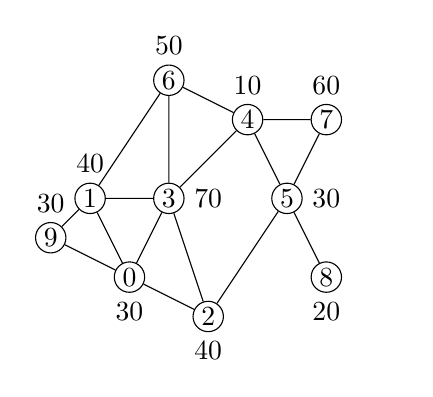
\begin{tikzpicture}
%      \draw [help lines] (0,-2) grid (4,2);
      \path [help lines] (0,-2) grid (4,2); 
      \node [vx, label=below:30]  (0) at (.5,-1) {0};
      \node [vx, label=above:40] (1) at (0, 0) {1};
      \node [vx, label=below:40] (2) at (1.5,-1.5) {2};
      \node [vx, label=right:70] (3) at (1, 0) {3};
      \node [vx, label=above:10] (4) at (2, 1) {4};
      \node [vx, label=right:30] (5) at (2.5, 0) {5};
      \node [vx, label=above:50] (6) at (1, 1.5) {6};
      \node [vx, label=above:60] (7) at (3, 1) {7};
      \node [vx, label=below:20] (8) at (3,-1) {8};
      \node [vx, label=above:30] (9) at (-.5,-.5) {9};
      \path [draw] 
      (0) -- (1)
      (0) -- (2)
      (0) -- (3)
			(0) -- (9)
      (1) -- (3)
      (1) -- (6)
			(1) -- (9)
      (2) -- (3)
      (2) -- (5)
      (3) -- (4)
      (3) -- (6)
      (4) -- (5)
      (4) -- (6)
      (4) -- (7)
      (5) -- (7)
      (5) -- (8);
    \end{tikzpicture}
}
  \\
  \subfloat[PCDG for Vertex 7]{
    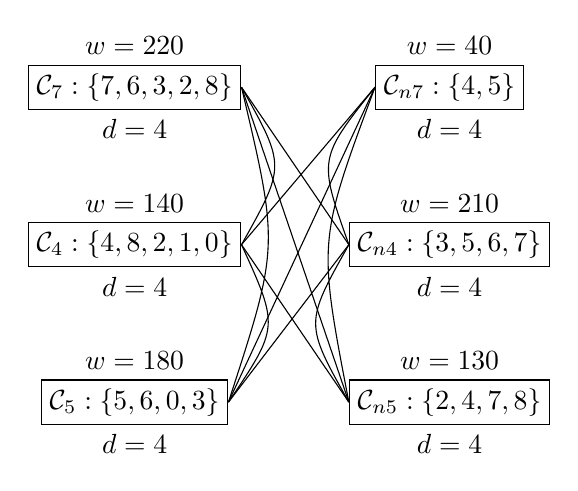
\begin{tikzpicture}
%      \draw [help lines] (0,-3) grid (6,3);
     \path [help lines] (0,-2) grid (4,2);
      \node [ex, label={above: $w=220$}, label={below: $d=4$}] (C7) at (1,2) {$\cC_7: \{7,6,3,2,8\}$};
      \node [ex, label={above: $w=40$}, label={below: $d=4$}] (CN7) at (5,2) {$\cC_{n7}: \{4,5\}$};
      \node [ex, label={above: $w=140$}, label={below: $d=4$}] (C4) at (1,0) {$\cC_4: \{4,8,2,1,0\}$};
      \node [ex, label={above: $w=210$}, label={below: $d=4$}] (CN4) at (5,0) {$\cC_{n4}: \{3,5,6,7\}$};
      \node [ex, label={above: $w=180$}, label={below: $d=4$}] (C5) at (1,-2) {$\cC_5: \{5,6,0,3\}$};
      \node [ex, label={above: $w=130$}, label={below: $d=4$}] (CN5) at (5,-2) {$\cC_{n5}: \{2,4,7,8\}$};

      \path [draw] 
      (C7.east) -- (CN5.west)
      (C7.east) -- (CN4.west)
      (CN4.west) -- (C5.east);
      \path [draw, decoration={bent, amplitude=16}, decorate]
      (C7.east) -- (C5.east)
      (C7.east) -- (C4.east)
      (C4.east) -- (C5.east);
      \path [draw]
      (CN7.west) -- (C5.east)
      (CN7.west) -- (C4.east)
      (CN5.west) -- (C4.east);
      \path [draw, decoration={bent, amplitude=-16}, decorate]
      (CN7.west) -- (CN5.west)
      (CN7.west) -- (CN4.west)
      (CN4.west) -- (CN5.west);
    \end{tikzpicture}
  }
  \end{center}
  \caption{Partial Cover Dependency Graph}
  \label{fig:pcdg}
\end{figure}


\subsubsection{PCDG Algorithm}
\label{sec:pcdg-alg}

The PCDG algorithm uses 2-hop information for immediate setup of the graph, as described in the previous section. After initial setup, the algorithm no longer updates any information beyond 1-hop. Figure~\ref{fig:pcdg-auto} shows the automaton for PCDG.

\begin{figure}[htp]
  \begin{center}
    \caption{Partial Cover Dependency Algorithm}
    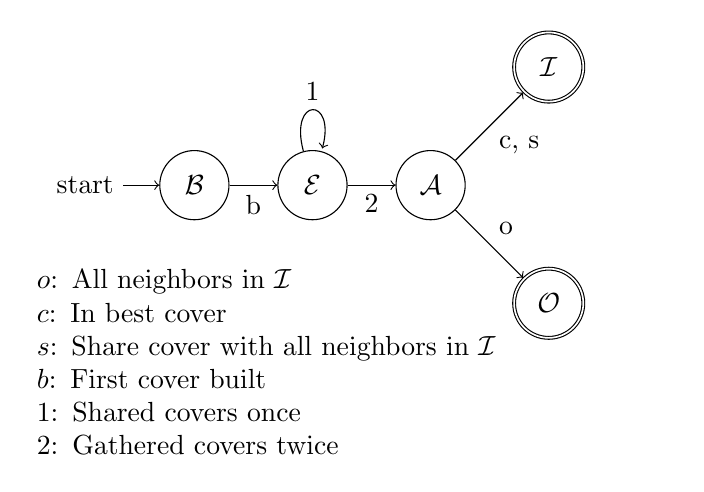
\begin{tikzpicture}
     % \draw[help lines] (0, -2) grid (5,2);
      \path [help lines] (0, -2) grid (5,2);
      \node [state, initial] (B) {\cBd};
      \node [state] (E) at (1.5, 0) {\cEd};
      \node [state] (A) at (3, 0) {\cAd};
      \node [state, accepting] (I) at (4.5, 1.5) {\cId};
      \node [state, accepting] (O) at (4.5, -1.5) {\cOd};

      \path [->] (B) edge node [below] {b} (E)
                 (E) edge node [below] {2} (A)
                     edge [loop above] node {1} ()
                 (A) edge node [above right]{o} (O)
                     edge node [below right]{c, s} (I);
      \node [text width=8cm] (key) at (2, -2.25) {
        $o$: All neighbors in \cId  \hspace{7cm}
        $c$: In best cover  \hspace{7cm}
        $s$: Share cover with all neighbors in \cId \hspace{5cm}
        $b$: First cover built  \hspace{7cm}
        $1$: Shared covers once  \hspace{7cm}
        $2$: Gathered covers twice  \hspace{4cm}};
                     
    \end{tikzpicture}
  \label{fig:red}
  \end{center}
\end{figure}

The bulk of the computational work for PCDG is done in the \cAd\ (Analyze) state. We assume that the covers in the Partial Cover Dependency Graph have been sorted according to degree, weight, and some sort of tie breaker. For the Dependency graph used in this paper, the priority order prefers lower weights, then higher degrees, and finally the covers unique id, as set during construction of the covers.

A node in the Analyze state will evaluate its highest priority cover. It can then turn on, turn off, or move onto the next priority cover. Algorithm~\ref{alg:pcdg} shows the general progress of the algorithm, and Algorithm~\ref{alg:pcdg-analyze} shows the specifics of this process.

This version of PCDG does very little analysis: if all neighbors are on, a node will turn off, otherwise, if a node is in it's current cover, the node will turn on. This keeps the communication cost low but sacrifices the quality of the solution. In future work we intend to explore other strategies for traversing the Graph.

In each communication round, each node sends it's current status to it's neighbors. Here another greedy choice is made, as shown in Algorithm~\ref{alg:pcdg-process}. If a neighbor turns on in a round, and that neighbor has the lowest battery of all neighbors which are on, then the node will attempt to find a cover containing itself and the neighbor node. In the next round this will be the highest priority cover. This strategy could also be modified. 

Our one-hop Algorithm performed surprising well against two-hop DEEPS when combined with the Redundancy Checking Algorithm and accounting for communication costs, as shown in Section~\ref{sub:netlife-results}.


\begin{algorithm}
\caption{PCDG Algorithm}
\begin{algorithmic}[1]
%\Require {$G(V,E)$: a Communicaton Network}
\ForAll {$v_u \in V$ in parrallel}
\Repeat
\Case [state]{}
\When [\cBd] {}
\State Build Covers
\State $state \gets \cE$
\When [\cEd] {}
\DoTimes [2]
\State Broadcast Covers \Comment to Neighbors
\State Add Covers \Comment from Neighbors
\EndTimes
\State $state \gets \cA$
\When [\cAd]
\State $state \gets$ {\scshape Analyze} \Comment see Procedure~\ref{alg:pcdg-analyze}
\When [\cId, \cOd]
\State $state \gets \cD$
\EndCase
\State Broadcast id, status
\ForAll {Neighbors $n$}
\State {\scshape Process}(n)  \Comment see Procedure~\ref{alg:pcdg-process}
\EndFor
\Until $state \equiv \cD$
\EndFor
\end{algorithmic}
\label{alg:pcdg}
\end{algorithm}

\begin{subalgorithms}
\begin{algorithm}
\caption{{\scshape Analyze}}
\begin{algorithmic}[1]
\Procedure {Analyze}{}
\If {no covers are available}
\If {$weight > 0$}
\State Turn On
\State $state \gets \cI$
\Else
\State Turn Off
\State $state \gets \cO$
\EndIf
\ElsIf {All Neighbors are On}
\State Turn Off
\State $state \gets \cO$
\ElsIf {This Node is in the Current Cover}
\State Turn On
\State $state \gets \cI$
\Else
\State Choose Next Cover
\State $state \gets \cA$
\EndIf
\State return $state$
\EndProcedure
\end{algorithmic}
\label{alg:pcdg-analyze}
\end{algorithm}

\begin{algorithm}
\caption{{\scshape Process}}
\begin{algorithmic}[1]
\Procedure {Process}{n}
\If {Self is Not on or off}
\If {$n$ is on}
\If {$weight(n) min(on neighbors)$}
\State Find of cover with n and self
\EndIf
\EndIf
\ElsIf {n is not on}
\State $state \gets \cA$
\EndIf 
\EndProcedure
\end{algorithmic}
\label{alg:pcdg-process}
\end{algorithm}
\end{subalgorithms}

\section{Simulation Software}
\label{sec:simulator}

We developed a discrete-event simulator in the Ruby programming language. Ruby was chosen primarily for its ''mix-in'' feature, weak typing, and simple unit-testing system. This allowed us to easily construct new families of nodes that used common simulation algorithms with very little code repetition.

The source code for each algorithm and the simulation framework are open source and available for download.\footnote{Using the mercurial VCS, command hg clone https://rvertex.graphcomplexity.googlecode.com/hg/ graphcomplexity-rvertex will retrieve a copy of the code repository. This paper uses revision 67446e3ca7 of the code base} 

The goal for this software package was to create a flexible, extensible platform for general simulation of distributed graph algorithms.Our approach for meeting this design goal was to attempt to modularize design as much as possible.

\section{Experiments}
\label{sec:experiments}
Experiments were conducted to test algorithm performance and examine the relationship between maximizing network lifetime and minimizing vertex cover.
\subsection{Minimum Weighted Vertex Cover}
\label{sub:mwvc-exp}

For the MWVC problem, we tested the DGMM algorithm against a similar algorithm developed in \cite{1582746}. The Koufogiannakis/Young algorithm uses a similar coin flipping mechanism between vertices, with each one choosing to be a 'root' or a 'leaf' node, and the algorithm proceeds in a way that guarantees that two adjacent nodes making independent decisions will reach the same conclusions. 

\subsection{Network Lifetime}

A key issue in developing algorithms in the Dependency Graph framework is the ranking of covers and the establishment of degrees. We chose a relatively simple method of ranking covers which has given good results. Most interesting, however, is that the initial ranking of covers seems to be superior to all subsequent rankings. This was determined during the experiment phase of our research, which is detailed in the next section.

Redundancy removal provides a tool to circumvent this problem. As each sensor reaches the end of its battery life, it can tell its neighbors to turn on. These neighbors can then negotiate with their neighbors, with redundant sensors turning off. The advantage of this approach is two-fold. First, there are no global reshuffle rounds. Communication costs are only incurred when strictly necessary to maintain the network. Second, sensors which are not affected by a particular event--those that are three or more hops away from a dying sensor--do not incur any extra cost as a result of a specific event.

Depending on the deployment details of a given network, communication costs may be much higher than sensing costs, so using redundancy checking as a means of network maintenance may extend network lifetimes. In Section~\ref{sub:netlife-results}, we explore this potential through simulation.

We chose the DEEPS algorithm developed in \cite{1640702}for target coverage and modified it suitably for vertex cover. This is a state-of-the art two-hop algorithm which has been demonstrated through simulation and real-world experiments to improve network lifetimes. DEEPS insures network coverage by assigning targets to sensor nodes, preferring the strongest member of weakest sets to take charge. 

DEEPS requires global reshuffles to maintain coverage, and those shuffles are proactive, they take place on a schedule rather than on an as needed basis.

\subsection{Experimental Design}
\label{sub:exp-design}
Random connected graphs were constructed, with the number of nodes and edges as the inputs. Nodes received a random weight between 400 and 1000. Graph construction proceeded by a modification of Erlang's method: all possible edges were generated and then random edges were chosen until the desired number of edges had been added to the graph. In order to ensure connectivity, Spanning Trees were constructed for each graph and connected together until each graph was a connected graph. 

For the MWVC problem, graphs were constructed with 120, 240, 480, and 960 vertices with average degrees of 3, 6, 12, 24, 48, and 96. 50 random graphs were generated at each size, and the Koufogiannakis/Young distributed algorithm\cite{1582746}, our distributed modification of the Gonzalez Generalized Maximal Matching Algorithm\cite{Gonzalez1995129}, and versions of each with the redundancy checking algorithm were run on each generated graph, with results being averaged.

For the Network Lifetime problem, the difficulty was to capture the communication cost associated with running the covering algorithms. We assume that in every case, a constant amount of energy is required to maintain the sensing and information sharing functions of the network. In our simulation, this cost is only applied to sensors that are ``on'' in a given round. The cost of re-organizing the sensors is a global cost, as every sensor in the network is required to participate in establishing a new vertex cover. This is applied as a constant drain on all sensors in the network. We conservatively simulate this drain as being on a spectrum from free to being equal to the cost of the information sharing and sensing function of the network. 

We tested PCDG and DEEPS in two scenarios: one where each algorithm performs a global reshuffle in each round, and one where each algorithm sets up an initial cover, and then uses redundancy checking to perform local maintenance on an as needed basis. Graphs were constructed with 20, 40, and 80 vertices and average degree of 3, 6, and 12. 25 experiments were run for each graph size.
 
\subsection{Experimental Results}
\label{sub:exp-results}
\subsubsection{Minimum Weighted Vertex Cover}
\label{sub:mwvc-results}
As expected, the addition of the constant time redundancy check improved results for both the DGMM algorithm and the K/Y algorithm. Figures~\ref{plt:match} and~\ref{plt:star} show the improvement. In our experiments the affect was small on average, less than 10\%, but this could be viewed as significant given the low cost of the routine. 
\begin{figure}[htp]
\begin{center}
\begin{tikzpicture}
  \begin{axis}[xlabel=Average Degree, ylabel=Total Weight, legend style={at={(1,0.25)}, anchor=east}, cycle list name={four} ]
    \addplot+[bls] table [x=links, y=mat-reg]{\averageone};
    \addplot+[bls] table [x=links, y=mat-reg]{\averagetwo};
    \addplot+[bls] table [x=links, y=mat-reg]{\averagethree};
    \addplot+[bls] table [x=links, y=mat-reg]{\averagefour};
    \addplot+[grt] table [x=links, y=mat-red]{\averageone};
    \addplot+[grt] table [x=links, y=mat-red]{\averagetwo};
    \addplot+[grt] table [x=links, y=mat-red]{\averagethree};
    \addplot+[grt] table [x=links, y=mat-red]{\averagefour};
    \legend{Match,,,, Match+R}
  \end{axis}
\end{tikzpicture}
\caption{Redundancy Applied to Matching}
\label{plt:match}
\end{center}
\end{figure}
\begin{figure}[htp]
\begin{center}
\begin{tikzpicture}
  \begin{axis}[xlabel=Average Degree, ylabel=Total Weight, legend style={at={(.95,0.75)}, anchor=north east}, cycle list name={four}]
    \addplot+[bls] table [x=links, y=star-reg]{\averageone};
    \addplot+[bls] table [x=links, y=star-reg]{\averagetwo};
    \addplot+[bls] table [x=links, y=star-reg]{\averagethree};
    \addplot+[bls] table [x=links, y=star-reg]{\averagefour};
    \addplot+[grt] table [x=links, y=star-red]{\averageone};
    \addplot+[grt] table [x=links, y=star-red]{\averagetwo};
    \addplot+[grt] table [x=links, y=star-red]{\averagethree};
    \addplot+[grt] table [x=links, y=star-red]{\averagefour};
    \legend{K/Y,,,, K/Y+R}
  \end{axis}
\end{tikzpicture}
\caption{Redundancy Applied to Koufogiannakis/Young}
\label{plt:star}
\end{center}
\end{figure}
More surprising was the difference in communication rounds between K/Y and DGMM. DGMM consistently resolved in one-tenth to one-third the number of communication rounds required by K/Y. Figure~\ref{plt:mwvc-rn} shows the difference in communication rounds required. The main reason for the difference is that in every communication round, DGMM is guaranteed to resolve each edge connected to one of a given node-pair in each round. The number of unresolved edges in the graph therefore quickly dwindles.

\begin{figure}[htp]
\begin{center}
\caption{Rounds to resolve MWVC}
\begin{tikzpicture}
  \begin{axis}[xlabel=Nodes + Link Density, ylabel=Communication Rounds, legend style={at={(0.5,.5)}, anchor=north}, legend columns=2]
    \addplot table [x=density, y=mat-reg]{\runs};
    \addplot table [x=density, y=star-reg]{\runs};
    \legend{Match, K/Y}
  \end{axis}
\end{tikzpicture}
\label{plt:mwvc-rn}
\end{center}
\end{figure}
The quality of solutions produced by K/Y and DGMM are similar. Figure~\ref{plt:mwvc-av} shows the quality of solutions between the two algorithms. K/Y holds an edge but that edge is slight.
  
\begin{figure}[htp]
\begin{center}
\begin{tikzpicture}
  \begin{axis}[xlabel=Average Degree, ylabel=Total Weight, legend style={at={(.95,.69)}, label={[font=\footnotesize]left:K/Y+R}, font=\footnotesize, anchor=south east}, legend columns=2, cycle list name={four-1-0}]
    \addplot+[grt] table  [x=links, y=star-red]{\averageone};
    \addplot+[grt] table  [x=links, y=star-red]{\averagetwo};
    \addplot+[grt] table  [x=links, y=star-red]{\averagethree};
    \addplot+[grt] table  [x=links, y=star-red]{\averagefour};
    \addplot+[inv] table [x=links, y=mat-red]{\averageone};
    \addplot+[inv] table [x=links, y=mat-red]{\averagetwo};
    \addplot+[inv] table [x=links, y=mat-red]{\averagethree};
    \addplot+[inv] table [x=links, y=mat-red]{\averagefour};
    \legend{(120),(240),(480),(960)}
  \end{axis}
  \begin{axis}[axis x line=none,axis y line=none, legend style={at={(.95,.68)}, label={[font=\footnotesize]left:DGMM+R}, font=\footnotesize, anchor=north east}, legend columns=2, cycle list name={four-0-1}]
    \addplot+[inv] table  [x=links, y=star-red]{\averageone};
    \addplot+[inv] table  [x=links, y=star-red]{\averagetwo};
    \addplot+[inv] table  [x=links, y=star-red]{\averagethree};
    \addplot+[inv] table  [x=links, y=star-red]{\averagefour};
    \addplot+[bls] table [x=links, y=mat-red]{\averageone};
    \addplot+[bls] table [x=links, y=mat-red]{\averagetwo};
    \addplot+[bls] table [x=links, y=mat-red]{\averagethree};
    \addplot+[bls] table [x=links, y=mat-red]{\averagefour};
    \legend{,,,,(120),(240),(480),(960)}
  \end{axis}
\end{tikzpicture}
\caption{Average Weights For MWVC}
\label{plt:mwvc-av}
\end{center}
\end{figure}


\subsubsection{Network Lifetime}
\label{sub:netlife-results}
When communication cost for network maintenance is considered to be negligible (or ignored), DEEPS outperforms PCDG by about 10\% in our simulations. Figure~\ref{plt:deeps-good} shows the performance of both algorithms in a communication cost free setting. DEEPS with reshuffle also outperformed DEEPS with redundancy checking when maintenance costs were considered to be free.
\begin{figure}[htp]
\begin{center}
\caption{Performance of Deeps}
\begin{tikzpicture}
  \begin{axis}[xlabel=Nodes * Link Density, ylabel=Lifetime, legend style={at={(1,0.25)}, anchor=east}]
    \addplot table [x=node_x_links, y=pcd]{\costless};
    \addplot table [x=node_x_links, y=deeps]{\costless};
    \legend{PCDG, DEEPS}
  \end{axis}
\end{tikzpicture}
\label{plt:match}
\end{center}
\end{figure}

PCDG using redundancy checking outperforms PCDG with global reshuffle regardless of the maintenance cost. Figure~\ref{plt:pcdg-comp} shows the performance of PCDG without maintenance costs.
\begin{figure}[htp]
\begin{center}
\begin{tikzpicture}
  \begin{axis}[xlabel=Average Degree, ylabel=Total Lifetime, legend style={at={(0.95,0.95)}, font=\footnotesize, anchor=north east}, cycle list name={three}]
    \addplot+[bls] table [x=links, y=pcd]{\steppingone};
    \addplot+[bls] table [x=links, y=pcd]{\steppingtwo};
    \addplot+[bls] table [x=links, y=pcd]{\steppingthree};
    \addplot+[grt] table [x=links, y=pcd]{\runningone};
    \addplot+[grt] table [x=links, y=pcd]{\runningtwo};
    \addplot+[grt] table [x=links, y=pcd]{\runningthree};
    \legend{PCDG (20),PCDG (40), PCDG (80), PCDG+R (20), PCDG+R (40), PCDG+R (80)}
  \end{axis}
\end{tikzpicture}
\caption{PCDG Without Communication Costs}
\label{plt:pcdg-comp}
\end{center}
\end{figure}


When communication costs are accounted for, the performance of DEEPS and PCDG improves when local reorganization using redundancy checking is used in place of global reshuffling. Figures~\ref{plt:deep-cost} and~\ref{plt:pcdg-cost} show how performance is affected by accounting for network maintenance.
\begin{figure}[htp]
\begin{center}
\begin{tikzpicture}
  \begin{axis}[xlabel=Cost, ylabel=Lifetime, legend style={at={(0.05,0.05)}, font=\footnotesize, anchor=south west},  cycle list name={three}]
    \addplot+[bls] table [x=cost, y=deeps_step]{\costcompone};
    \addplot+[bls] table [x=cost, y=deeps_step]{\costcomptwo};
    \addplot+[bls] table [x=cost, y=deeps_step]{\costcompthree};
    \addplot+[inv] table [x=cost, y=deeps_run]{\costcompone};
    \addplot+[inv] table [x=cost, y=deeps_run]{\costcomptwo};
    \addplot+[inv] table [x=cost, y=deeps_run]{\costcompthree};
    \legend{DEEPS (20),DEEPS (40),DEEPS (80)}
  \end{axis}
  \begin{axis}[axis x line=none, axis y line=none, legend style={at={(0.95,0.95)}, font=\footnotesize, anchor=north east},  cycle list name={three}]
    \addplot+[inv] table [x=cost, y=deeps_step]{\costcompone};
    \addplot+[inv] table [x=cost, y=deeps_step]{\costcomptwo};
    \addplot+[inv] table [x=cost, y=deeps_step]{\costcompthree};
    \addplot+[grt] table [x=cost, y=deeps_run]{\costcompone};
    \addplot+[grt] table [x=cost, y=deeps_run]{\costcomptwo};
    \addplot+[grt] table [x=cost, y=deeps_run]{\costcompthree};
    \legend{,,,DEEPS+R (20),DEEPS+R (40),DEEPS+R (80)}
  \end{axis}
\end{tikzpicture}
\caption{Deeps with Communication Costs}
\label{plt:deep-cost}
\end{center}
\end{figure}

\begin{figure}[htp]
\begin{center}
\begin{tikzpicture}
  \begin{axis}[xlabel=Cost, ylabel=Lifetime, legend style={at={(0.05,0.05)}, font=\footnotesize, label={[font=\footnotesize]above:PCDG}, anchor=south west}, cycle list name={three}]
    \addplot+[bls] table [x=cost, y=pcd_step]{\costcompone};
    \addplot+[bls] table [x=cost, y=pcd_step]{\costcomptwo};
    \addplot+[bls] table [x=cost, y=pcd_step]{\costcompthree};
    \addplot+[inv] table [x=cost, y=pcd_run]{\costcompone};
    \addplot+[inv] table [x=cost, y=pcd_run]{\costcomptwo};
    \addplot+[inv] table [x=cost, y=pcd_run]{\costcompthree};
    \legend{(20),(40),(80)}
  \end{axis}
  \begin{axis}[xlabel=Cost, ylabel=Lifetime, legend style={at={(0.95,0.65)}, font=\footnotesize, label={[font=\footnotesize]left:PCDG+R}, anchor=north east}, cycle list name={three}]
    \addplot+[inv] table [x=cost, y=pcd_step]{\costcompone};
    \addplot+[inv] table [x=cost, y=pcd_step]{\costcomptwo};
    \addplot+[inv] table [x=cost, y=pcd_step]{\costcompthree};
    \addplot+[grt] table [x=cost, y=pcd_run]{\costcompone};
    \addplot+[grt] table [x=cost, y=pcd_run]{\costcomptwo};
    \addplot+[grt] table [x=cost, y=pcd_run]{\costcompthree};
    \legend{,,,(20),(40),(80)}
  \end{axis}
\end{tikzpicture}
\caption{PCDG with Communication Costs}
\label{plt:pcdg-cost}
\end{center}
\end{figure}

\bibliography{../IPDPS_2010/vertex_bib}
\end{document}
% LocalWords:  Koufaganis
